%************************************************
\myChapter{Oprogramowanie}\label{ch:software}
%************************************************

Jako zwolennik wolnego i otwartego oprogramowania starałem się korzystać tylko i wyłącznie z takich właśnie narzędzi.

\graffito{ \includegraphics[width=\marginparwidth]{gfx/gnuhead_inkscape.pdf} Logo Fundacji Wolnego Oprogramowania \ppauza Free Software Foundation \citep{FSF}}Sama praca udostępniana jest na zasadach otwartej licencji \textsc{GNU GPL 3.0}. Wszystkie otwarte licencje typu \textsc{GNU GPL} stworzone zostały przez fundację FSF, która też stoi na straży ich przestrzegania.

Oprogramowanie stworzone na potrzeby pracy składa się z dwóch elementów:
\begin{itemize}
 \item oprogramowania na komputer,
 \item oprogramowania na mikrokontroler.\\
\end{itemize}

Większość zmian mikrokontrolera, opisywana w rozdziale \ref{ch:hardware}, pociągała za sobą przepisanie oprogramowania praktycznie od zera ze względu na rdzenie z kompletnie innych rodzin, inne dostępne moduły oraz inny sposób ich obsługi. Ilość tych zmian, a także dodatkowe utrudnienia pod postacią niedostępności debugowania, skomplikowanej instalacji słabo dostępnych i przestarzałych pakietów kompilatora skłoniły mnie do poszukania rozwiązania typu RTOS lub podobnego.
W taki sposób znalazłem środowisko \textsc{Energia}, \textit{fork} środowiska \textsc{Arduino}\graffito{Programy w środowisku \textsc{Arduino} noszą nazwę ,,sketch''.}, oparty o toolchain \textsc{msp-gcc} oraz \textsc{arm-gcc}, pozwalający pisać programy w języku C++ ukrywając wiele szczegółowych operacji przed programistą jak np. konfiguracja stosu USB, pozwalając mu skoncentrować się na istocie tworzonego programu.\\

\section{Protokół komunikacji}

Komunikacja hosta z mikrokontrolerem odbywa się przez wirtualny port szeregowy (urządzenie \textsc{USB Communications Device Class, CDC}). Narzuca to kilka ograniczeń dotyczących możliwości protokołu, które należy uwzględnić podczas jego projektowania:
\begin{itemize}
 \item mikrokontroler będzie widoczny jako zwykłe urządzenie znakowe, należy więc zadbać, aby przesyłane dane były w postaci czytelnej także w zwykłym kliencie terminala,
 \item sposób komunikacji musi uwzględniać możliwość synchronizacji, np. za pomocą specjalnego znaku, który nie pojawia się w innym przypadku,
 \item protokół musi być możliwie zwięzły ze względu na ograniczoną przepustowość łącza,
 \item komunikacja musi przebiegać dwukierunkowo (w trybie przynajmniej half-duplex).\\
\end{itemize}

Uwzględniając powyższe wytyczne, opracowałem protokół o następujących cechach:
\begin{itemize}
 \item Wszystkie przesyłane dane są pod postacią znaków kodu ASCII, zarówno z hosta do mikrokontrolera jak i z powrotem. Używane są trzy sposoby tłumaczenia danych z postaci binarnej na kod ASCII:
 \begin{enumerate}
  \item Numeryczny zapis dziesiętny\label{item:decimal} \pauza wartości zapisywane są w~systemie dziesiętnym po jednej stronie, druga strona konwertuje liczbę ponownie na system binarny.
  \item Base64\label{item:base64} \pauza System konwersji danych konwertujący ciąg 8-bitowych danych na ciąg 6-bitowych danych z określonym alfabetem. Algorytm ten opisany jest w sekcji~\ref{sec:base64}.
  \item Zapis binarny z offsetem\label{item:offset} \pauza dla ograniczonych wielkości zmiennych zastosowałem przesunięcie wartości, które zapewnia ich prezentację w kodzie ASCII: do wartości zmiennej dodawany jest offset 'a', tak więc 'a' rozumiane jest jako 0, 'b' jako 1, itd.
 \end{enumerate}
 \item Do synchronizacji wykorzystany został znak o kodzie \textsc{0x0D}, czyli powrót karetki (\textit{carriage return}), dzięki czemu synchronizacja jest czytelnia zarówno dla komputera jak i człowieka.
 \item Protokół został zaprojektowany w modelu klient-serwer, gdzie klient (komputer) odpytuje o dane serwer (mikrokontroler).\\
\end{itemize}

O wyborze algorytmu Base64 (\ref{item:base64}) zadecydowała jego powszechność, co przekłada się na dostępność narzędzi kodujących i dekodujących.
Biblioteki \texttt{Qt} także dostarczają implementacji funkcji obsługujących to kodowanie.

Prostota tego algorytmu przekłada się na możliwość stworzenia zoptymalizowanej implementacji, która na mikrokontrolerze może znacząco się przekładać na szybkość transmisji danych.

Dodatkowo, dla pewnych struktur danych, nawet w postaci zakodowanej można szybko ocenić czy są one poprawne.\\

Dzięki identyfikowaniu się urządzenia jako port szeregowy, możliwe jest podłączenie się dowolnym klientem terminala (np. \textsc{screen}, \textsc{minicom}, itp.) i ręczna obsługa urządzenia.
Znacznie pomaga to podczas rozwijania oprogramowania umożliwiając łatwe wprowadzenie systemu w~skrajne przypadki.\\

Obsługę protokołu od strony mikrokontrolera można przedstawić pseudokodem z algorytmów~\ref{alg:proto_uc_interrupt}~i~\ref{alg:proto_uc_main}.
\begin{algorithm}
\caption{Obsługa protokołu komunikacji, strona mikrokontrolera, przerwanie portu szeregowego}
\label{alg:proto_uc_interrupt}
\begin{algorithmic}[1]
  \REQUIRE \texttt{dane} \ppauza tablica statyczna, do której końca dopisywane są przychodzące dane. Wystarczająco duża na pomieszczenie spodziewanej ilości danych.\\
  \texttt{Serial} \ppauza obiekt klasy obsługującej port szeregowy\\
  \texttt{input, length, commandReady} \ppauza zmienne wykorzystywane do synchronizacji pomiędzy obsługą przerwania, a główną pętlą programu
  \STATE count \textleftarrow{} $0$
  \WHILE{Serial.available()}
    \IF{commandReady == true}
      \STATE continue;
    \ENDIF
    \STATE char \textleftarrow{} Serial.read()
    \STATE dane[count++] \textleftarrow{} char
    \IF{char == '\textbackslash{}r'}
      \STATE length \textleftarrow{} count
      \STATE input \textleftarrow{} dane
      \STATE count \textleftarrow{} $0$
      \STATE commandReady \textleftarrow{} true
    \ENDIF
  \ENDWHILE
\end{algorithmic}
\end{algorithm}

\begin{algorithm}
\caption{Obsługa protokołu komunikacji, strona mikrokontrolera, główna pętla}
\label{alg:proto_uc_main}
\begin{algorithmic}[1]
  \REQUIRE \texttt{Serial} \ppauza obiekt klasy obsługującej port szeregowy\\
  \texttt{input, length, commandReady} \ppauza zmienne wykorzystywane do synchronizacji pomiędzy obsługą przerwania, a główną pętlą programu\\
  \texttt{toBase64(input, output, inputLength)} \ppauza funkcja zamieniająca ciąg danych \texttt{input} o długości \texttt{inputLength} na kodowanie Base64 i zapisująca wynik do \texttt{output}, zwracająca długość ciągu \texttt{output}\\
  \texttt{handleCommand(input, output)} \ppauza funkcja obsługi komend protokołu, zapisuje ewentualne dane zwrotne w buforze \texttt{output}, zwraca długość zapisanych danych
  \WHILE{true}
    \IF{commandReady == true}
      \STATE resultLength \textleftarrow{} handleCommand(input, commandBuffer)
      \STATE b64Length \textleftarrow{} toBase64(commandBuffer, outputBuffer, resultLength)
      \STATE Serial.write(outputBuffer, b64Length)
      \STATE Serial.write('\textbackslash{}r')
      \STATE commandReady \textleftarrow{} false
    \ENDIF
  \ENDWHILE
\end{algorithmic}
\end{algorithm}

\subsection{Dostępne komendy}

Wszystkie komendy identyfikowane są pierwszą literą, mogą mieć zmienną liczbę argumentów, kończą się znakiem carriage return, a błędne komendy są odrzucane.
Dostępne komendy protokołu wraz z ich opisem przedstawione są poniżej.
\newline
\newline
\textsl{a}
Komenda postaci \texttt{a\#\#} zapalająca wybrany moduł, gdzie \texttt{\#\#} oznacza numer nadajnika do zapalenia, kodowany zapisem dziesiętnym (\ref{item:decimal}).
\newline
\newline
\textsl{e}
Komenda postaci \texttt{e\#\#} wybierająca do odczytania zadany moduł, gdzie \texttt{\#\#} oznacza numer modułu do wybrania, kodowany zapisem dziesiętnym (\ref{item:decimal}).
\newline
\newline
\textsl{r}
Komenda postaci \texttt{r} dokonująca odczytu z wybranego aktualnie modułu, stosowana zwykle w połączeniu z komendami \textsl{a} i \textsl{e}.

Zwracane są dane postaci \texttt{rxya}, gdzie \texttt{x} to numer wybranego aktualnie nadajnika, \texttt{y} to numer wybranego aktualnie modułu odbierającego, \texttt{a} to bajt zawierający dane zwrócone przez ten modul, wszystko zakodowane zakodowane Base64 (\ref{item:base64}).
\newline
\newline
\textsl{d}
Komenda postaci \texttt{d\#\#} ustawiająca czas oczekiwania \textsl{delay} na zadany argument \texttt{\#\#}, kodowany zapisem dziesiętnym (\ref{item:decimal}).
\newline
\newline
\textsl{D}
Komenda postaci \texttt{D} wyświetlająca (w postaci czytelnej dla człowieka) aktualną wartość zmiennej \textsl{delay}.
\newline
\newline
\textsl{p}
Komenda postaci \texttt{pxabc} zapalająca wybrany moduł i pobierająca kompletny zestaw odczytów, gdzie \texttt{x} oznacza numer nadajnika do zapalenia, zaś \texttt{abc} to ciąg odbiorników, z których dane należy pobrać. Wszystkie argumenty kodowane są zapisem z offsetem (\ref{item:offset}). Pomiędzy wybraniem modułu do odczytania, a dokonaniem odczytu, odczekiwane jest \textsl{delay} mikrosekund.

Zwracane są dane zakodowane w postaci \texttt{pxabc}, gdzie \texttt{x} to numer nadajnika, \texttt{abc} to ciąg bajtów odczytanych z zadanych odbiorników, wszystkie dane zakodowane Base64 (\ref{item:base64}).
\newline
\newline
\textsl{t}
Komenda postaci \texttt{t} zmieniająca stan diody niebieskiej. Używana do weryfikacji poprawnego przetwarzania komend.

\section{Oprogramowanie na komputer}
W celu stworzenia oprogramowania dla komputera wykorzystałem kilka środowisk i bibliotek.

\paragraph{Qt}
Wieloplatformowe środowisko (ang. \textsl{framework}) \textsmaller{Qt}, licencjonowane wolną licencją \textsc{GNU LGPL 2.1} oraz \textsc{GNU GPL 3.0}, składa się z kilku komponentów.
W jego skład wchodzą między innymi: biblioteka \textsc{Qt} oraz kompilator \verb|moc|.
Wszystkie te elementy znacznie usprawniają pisanie aplikacji w języku \verb|C++| dostarczając metod, które abstrahują od specyfiki wykorzystywanego systemu operacyjnego.

Pisanie nawet skomplikowanych programów z wykorzystaniem \textsc{Qt} jest proste, łatwe, szybkie i przyjemne.
Programista świadomy różnic pomiędzy systemami operacyjnymi i delegujący obsługę parametrów do metod dostarczanych przez klasy bibliotek \textsc{Qt} zyskuje możliwość skompilowania swojego kodu pod platformy \textsc{Linux}, \textsc{Windows} oraz \textsc{Mac OS X} bez konieczności jakichkolwiek zmian.

Szerokie spektrum dostarczanych klas (począwszy od kontenerów danych i metod iteracji, przez obsługę urządzeń wejściowych, przez obsługę sieci, aż po rysowanie i zarządzanie grafikami i wiele, wiele innych\ldots) zapewnia, że do zaimplementowania wielu aplikacji nie będzie wymagane wykorzystanie bibliotek trzecich.
\newline
\newline
\textsl{Sygnały i sloty}
Ze względu na intensywne wykorzystywanie w stworzonych aplikacjach połączeń sygnał-slot, zamieszczam poniżej ich opis.

Centralną właściwością środowiska \textsc{Qt}, a jednocześnie jedną z najbardziej odróżniających ten framework od innych, jest mechanizm sygnałów i slotów będący zarządzaną metodą komunikacji pomiędzy obiektami.

Chociaż na pierwszy rzut oka przypomina ona znane dotychczas metody oparte o wywołania zwrotne (ang. \textsl{callback}) i faktycznie się z~nich wywodzi, to jednak różni się od nich w kilku kluczowych aspektach.

Jest to metoda dynamiczna (działająca w czasie wykonywania \ppauza ang. \textsl{runtime}).
Metoda wywołań zwrotnych wykorzystywana jest głównie do zamodelowania statycznych (tj. znanych już podczas czasu kompilacji \ppauza ang. \textsl{compiletime}) powiązań pomiędzy obiektami jak np:
\begin{verse}
użytkownik kliknął przycisk \texttimes~\textrightarrow~wywołaj metodę \texttt{close()}
\end{verse}

W przypadku tym przypisuje się wskaźnik do funkcji do pewnego pola klasy wywołującej, który w momencie zajścia zdarzenia jest wywoływany.
Konsekwencją takiego podejścia jest konieczność znania odbiorników w czasie kompilacji, co uniemożliwia np. ładowanie wtyczek w czasie rzeczywistym i powiadamiania ich o zdarzeniach w następujący sposób:
\begin{verse}
powiadom wszystkie odbiorniki o zajściu zdarzenia $\omega$
\end{verse}

Zastosowanie w tym miejscu wektorów wskaźników jest jedynie obejściem problemu, a nie jego rozwiązaniem, gdyż nakłada na programistę obowiązek pamiętania o poprawnym przydzielaniu i zwalnianiu pamięci na te elementy, w przypadku aplikacji wielowątkowych szczegółowego analizowania zależności czasowych pomiędzy wywołaniami kodu obiektów, oraz drobiazgowego sprawdzania typów wywołań.

Podejście to wprowadza ponadto nadmiarową i zbędną wiedzę o~odbiornikach do nadajnika.

Rozwiązanie dostarczane przez framework \textsc{Qt} jest elegancką metodą pozbycia się wymienionych wad na rzecz udostępnienia programiście prostego w obsłudze, lecz potężnego i skutecznego, mechanizmu dynamicznego wiązania obiektów w pary nadajnik-odbiornik.

Przekazywane sygnały są ,,wątkowo-bezpieczne'' (ang. \textsl{thread-safe}), co pozwala na przetwarzanie sygnału w innym wątku niż ten, który zainicjował jego wysłanie.
Aby zrealizować takie podejście, każdy z~obiektów dziedziczących po klasie \verb|QObject| powinien należeć do jakiegoś wątku, tak aby był on uwzględniany w pętli zdarzeń (ang. \textsl{event loop}), jaka jest przez ten wątek przetwarzana.
Domyślnie każdy nowy obiekt przynależy do wątku rodzica, który go utworzył.

Pociąga to za sobą konsekwencję, że jeżeli obiekt nie przynależy do żadnego wątku, to jego zdarzenia nie będą przetwarzane.

W celu uproszczenia obsługi, środowisko \textsc{Qt} domyślnie wykorzystuje do wszystkich obiektów wątek główny aplikacji i jeśli programista jawnie nie usunie z niego obiektów, to ich sygnały będą przetwarzane właśnie w tym wątku.

Aby zintegrować to rozwiązanie z kodem, postanowiono ,,rozszerzyć'' standard\graffito{,,Rozszerzenie'' to wykorzystywane jest tylko i wyłącznie do środowiskia \textsc{Qt}.} języka \verb|C++|.
Do istniejących już kwalifikatorów \verb|public|, \verb|private| i~\verb|protected| dodano dwa nowe: \verb|signals| i \verb|slots|.

Kwalifikator \verb|signals| definiuje sygnały. Mają one taką samą strukturę, jak zwykłe metody klasy z następującymi wyjątkami:
\begin{aenumerate}
  \item definicja sygnału jest tylko i wyłącznie jego deklaracją, oznacza to, że sygnał nie posiada żadnego kodu, jest tylko abstrakcyjnym tworem komunikującem zajście pewnego zdarzenia,
  \item sygnały nie mogą zwracać wartości \ppauza zwracanym typem musi być \verb|void|, a wszelkie przekazywane dane zawarte są w argumentach,
  \item sygnały są zawsze publiczne.
\end{aenumerate}

Deklarację pewnej minimalnej klasy zawierającej sygnały prezentuje listing \ref{lst:signals_declaration}.

\begin{listing}
  \lstinputlisting{listings/signals_declaration.cpp}
  \caption{Klasa zawierająca sygnały}
  \label{lst:signals_declaration}
\end{listing}

Jak pokazano, aby klasa mogła wykorzystać mechanizm sygnałów (a także slotów), musi ona dziedziczyć z klasy \verb|QObject| i wywoływać makro \verb|Q_OBJECT| w prywatnej części deklaracji.

Kwalifikator \verb|slots|, jak łatwo się domyślić, deklaruje sloty.
Poza dodatkową możliwością wywołania slotu, są to tradycyjne metody klasy i tak samo obowiązują je pozostałe kwalifikatory: \verb|public|, \verb|private| i~\verb|protected|.
W odróżnieniu od sygnałów, sloty wymagają dostarczenia implementacji i mogą zwracać wartości.

Deklarację pewnej minimalnej klasy zawierającej sloty prezentuje listing \ref{lst:slots_declaration}.

\begin{listing}
  \lstinputlisting{listings/slots_declaration.cpp}
  \caption{Klasa zawierająca sloty}
  \label{lst:slots_declaration}
\end{listing}

Połączenie emitera ze słuchaczem następuje poprzez wywołanie metody \verb|connect| klasy \verb|QObject|, której argumentami są obiekty nadający i~odbierający, a także nazwy łączonych metod.
Sygnatura slotu i sygnału musi być taka sama, z wyjątkiem zwracanego typu.

Użyteczną cechą jest możliwość podłączenia sygnału do sygnału, dzięki czemu zostanie wywołany drugi z sygnałów, a w efekcie podłączone do niego sloty.

Pozostała charakterystyka tego rozwiązania, taka jak przekazywanie meta-typów, rozgraniczenie pomiędzy obiektem nadającym, a odbierającym oraz inne, nie została wykorzystana w stworzonym oprogramowaniu, w związku z czym odsyłam czytelnika do dokumentacji środowiska \textsc{Qt} \citep{Qt}.
\newline
\newline
\textsl{Kompilator moc} Ponieważ powyższe rozwiązanie nie należy do standardu języka \verb|C++|, zaś całe oprogramowanie stworzone przy pomocy środowiska \textsc{Qt} kompilowane jest przy pomocy kompilatora \verb|C++| zgodnego ze standardem ISO/IEC C++\citep{CPPStandard}, takiego jak \texttt{g++}, dostarczany jest wraz z \textsc{Qt} kompilator \texttt{moc}, czyli \textsl{meta-object compiler}.

Zadaniem tego narzędzia jest przeparsowanie dostarczonych plików źródłowych pod kątem odszukania wśród nich deklaracji klas dziedziczących z \verb|QObject|, a zatem wykorzystujących rozszerzone możliwości oferowane przez \textsc{Qt} i wygenerowanie kodu zrozumiałego przez wspomniany wyżej ,,zwykły'' kompilator.
Kod dostarczony przez programistę, pozbawiony rozszerzeń \textsc{Qt} oraz kod wygenerowany przez narzędzie \texttt{moc} są kompilowane, a następnie łączone ze sobą na etapie linkowania.

\paragraph{QSerialPort}
Biblioteka \textsc{QSerialPort}, oparta o wolną licencję \textsc{GNU LGPL 2.1}, dostarcza metod komunikacji wykorzystujących port szeregowy.
Opiera się ona o środowisko \textsc{Qt}, przez co bardzo łatwo jest zintegrować ją z projektami korzystającymi z tych narzędzi.
Podobnie jak samo \textsc{Qt}, biblioteka ta jest wieloplatformowa, co było jednym z~głównych powodów, dla których wybrałem właśnie ją.

Dostarcza ona metody obsługi portów oparte o interfejs \verb|QIODevice| udostępniany przez \textsc{Qt}, które implementowane są z wykorzystaniem natywnych funkcji systemowych dla każdej z platform, dzięki czemu przekazywanie danych odbywa się szybko i sprawnie \citep{QSP}.

\subsection{RayDisplay}

Program obsługujący urządzenie od strony komputera nosi nazwę \texttt{RayDisplay}.

Składa się on z klas:
\begin{itemize}
 \item \verb|RayDisplayWindow| \pauza klasa dziedzicząca po \verb|QMainWindow|, implementująca interfejs użytkownika,
 \item \verb|RayDisplayScene| \pauza klasa dziedzicząca po \verb|QGraphicsScene|, implementująca algorytm heatmapy,
 \item \verb|CommunicationThread| \pauza klasa dziedzicząca po \verb|QThread|, implementująca komunikację z portem szeregowym.\\
\end{itemize}

Program rozpoczyna swoje działanie od stworzenia interfejsu użytkownika, co oznacza stworzenie obiektu typu \verb|RayDisplayWindow|.
Tworzy on okienko, za pomocą którego użytkownik będzie mógł kontrolować i monitorować działanie urządzenia.

Rysunek \ref{fig:raydisplay} pokazuje program po uruchomieniu.

\begin{figure}
 \centering
 \makebox[\textwidth][r]{
  \resizebox{.85\largefigure}{!}{
   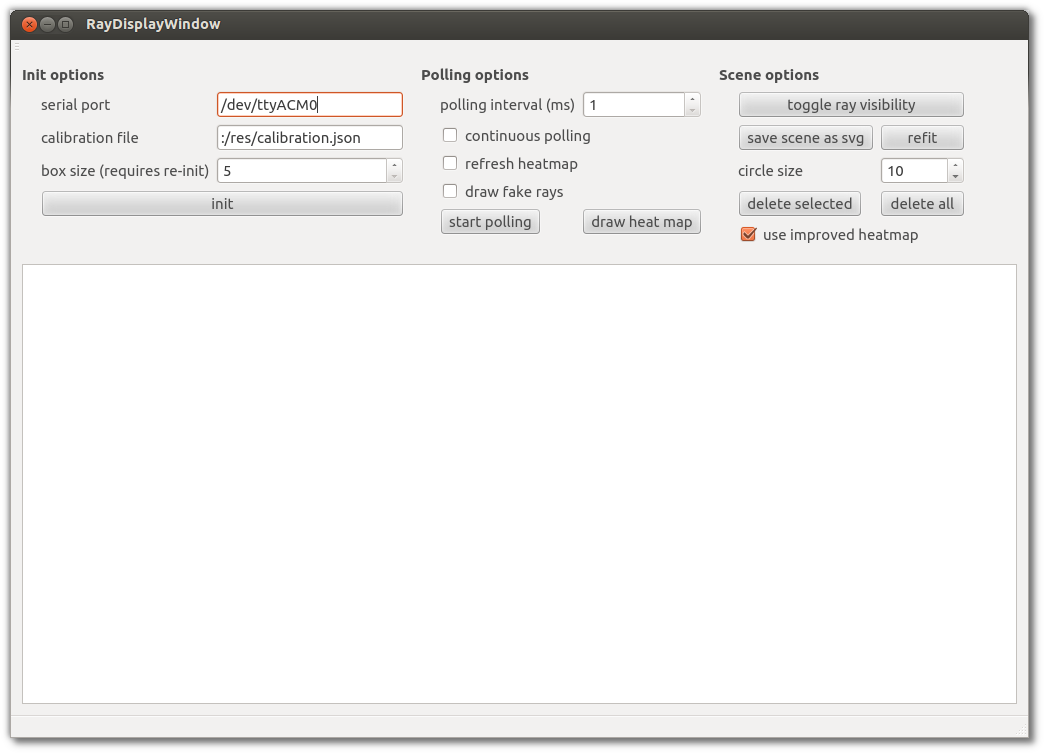
\includegraphics[width=\textwidth]{gfx/RayDisplay}
  }
 }
 \caption{Uruchomiony program RayDisplay}
 \label{fig:raydisplay}
\end{figure}

Po kliknięciu na przycisk {\fbox{\texttt{init}}} tworzone są pojedyncze obiekty klas \verb|RayDisplayScene| oraz \verb|CommunicationThread|, usuwając najpierw ewentualnie istniejące poprzednie ich instancje.

Gdy obiekty te zostaną już stworzone, łączone są ze sobą wszystkie sygnały i sloty, umożliwiając przesyłanie danych pomiędzy metodami programu.

Klasa \verb|RayDisplayScene| podczas inicjalizacji tworzy reprezentację ramki oraz elementy algorytmu heatmapy.

W dalszej kolei instancja \verb|CommunicationThread| tworzy nowy wątek, w którym otwiera port szeregowy, zaczyna oczekiwać powiadomienia o żądaniu pobrania danych.

Teraz użytkownik powinien kliknąć na przycisk \fbox{\texttt{start polling}}, ewentualnie zaznaczając wcześniej opcję \texttt{continuous polling}, która sprawi, że po otrzymaniu jednej porcji danych, natychmiast zostanie wysłanie żądanie o kolejną.

Dane odebrane przez \verb|CommunicationThread| są przekazywane sygnałem do \verb|RayDisplayWindow|, gdzie następuje ich wstępna analiza, po czym przekazywane są do \verb|RayDisplayScene| w postaci unormowanej.
Krok ten pozwala ograniczyć liczbę potrzebnych metod służących do obsługi danych pobieranych różnymi sposobami.\\

Istotne jest, że komunikacja z urządzeniem zachodzi w osobnym wątku, nie obciążając tym samym wątku głównego zwanego przez \texttt{Qt} wątkiem GUI, gdyż jest to jedyny wątek, który może malować interfejs użytkownika.

Charakterystyka używanego portu szeregowego wymaga ciągłego odpytywania o nowe dane, w przeciwnym wypadku mogą one zostać utracone.

Pętla taka w głównym wątku wpływałaby negatywnie na obsługę wydarzeń związanych z obsługą interfejsu, co mogłoby skutkować w ostateczności oznaczeniem przez system aplikacji jako nieodpowiadającej na zdarzenia.

Podejście takie wymaga jednak synchronizacji żądań i odpowiedzi, co zostało wykonane z pomocą wzorca producent\pauza{}konsument, gdzie bufor żądań strzeżony jest dwoma semaforami\graffito{Semafor to licznik z dostępem atomowym służący do synchronizacji wątków}: piszącym i czytającym.

Ponieważ \verb|CommunicationThread| nie używa pętli zdarzeń (\textsl{event loop}), nie jest możliwe przesyłanie do niego żądań za pomocą slotów. Może on mimo tego emitować sygnały, zostało to wykorzystane do przesyłu danych do dalszego przetwarzania.

Gwarantuje to obsłużenie nowych danych możliwie szybko zachowując przy tym poprawne przetwarzanie zdarzeń z pętli.\\

Program umożliwia także ustawianie, przesuwanie i usuwanie sztucznych, wirtualnych przeszkód, które umożliwiają testowanie algorytmu bez względu na jakość otrzymywanych danych.

Podczas działania programu, użytkownikowi prezentowany jest szereg opcji wpływających na działanie programu:
\begin{itemize}
 \item \fbox{polling interval} wartość interwału pomiędzy odebraniem danych o wysłaniem żądania kolejnej ich porcji, wyrażony w milisekundach,
 \item opisana powyżej opcja \fbox{continuous polling},
 \item \fbox{refresh heatmap} opcja włączająca odświeżanie heatmapy po każdej porcji danych,
 \item \fbox{draw fake rays} powodujący włączenie kolizji z wirtualnymi przeszkodami,
 \item \fbox{draw heatmap} wymuszający odświeżenie heatmapy (np. gdy wyłączone jest jej automatyczne odświeżanie),
 \item \fbox{toggle ray visibility} przełącza widoczność promieni, pozwala to na podgląd heatmapy bez zasłaniających linii,
 \item \fbox{save scene as svg} zapisuje widoczną scenę do pliku \texttt{scene.svg} w katalogu roboczym aplikacji,
 \item \fbox{refit} pozwala przeskalować scenę do aktualnych rozmiarów okna (zachowując proporcje),
 \item \fbox{circle size} rozmiar stawianych wirtualnych przeszkód,
 \item \fbox{delete selected} i \fbox{delete all} usuwające wirtualne przeszkody, odpowiednio: zaznaczone i wszystkie,
 \item \fbox{use improved heatmap} wybierający podstawowy lub ulepszony algorytm heatmapy.
\end{itemize}

Obsługa wirtualnych przeszkód odbywa się za pomocą myszki:
\begin{itemize}
 \item prawy przycisk ustawia nową przeszkodę o rozmiarze zadanym w opcjach programu,
 \item lewy przycisk umożliwia wybieranie i przesuwanie.
\end{itemize}
